\documentclass{article}
\usepackage{xcolor}
\usepackage{titleps}
\usepackage[letterpaper, margin=0.95in]{geometry}
\usepackage{url}
\usepackage{amsmath}
\usepackage{amssymb}
\usepackage{wrapfig}
\usepackage{float}
\usepackage{mathtools}
\usepackage{enumitem}
\usepackage{tabu}
\usepackage{parskip}
\usepackage{natbib}
\usepackage{listings}
\usepackage{tikz}
\usepackage{quiver}

\usepackage{graphicx}
\usepackage{caption}
\usepackage{subcaption}
\usepackage[export]{adjustbox}
\usepackage{hyperref}

\newcommand{\xb}{\mathbf{x}}
\newcommand{\yb}{\mathbf{y}}
\newcommand{\wb}{\mathbf{w}}
\newcommand{\Xb}{\mathbf{X}}
\newcommand{\Yb}{\mathbf{Y}}
\newcommand{\tr}{^T}
\newcommand{\hb}{\mathbf{h}}
\newcommand{\Hb}{\mathbf{H}}

\DeclareFontShape{OT1}{cmtt}{bx}{n}{<5><6><7><8><9><10><10.95><12><14.4><17.28><20.74><24.88>cmttb10}{}


\usepackage{forest}

\usepackage{hyperref}
\usepackage[color=red]{todonotes}
\usepackage{forest}
\definecolor{light-yellow}{HTML}{FFE5CC}

\usepackage{cleveref}

\newpagestyle{ruled}
{\sethead{Berkeley CS 285}{Deep Reinforcement Learning, Decision Making, and Control}{Fall 2023}\headrule
  \setfoot{}{}{}}
\pagestyle{ruled}

\renewcommand\makeheadrule{\color{black}\rule[-.75\baselineskip]{\linewidth}{0.4pt}}
\renewcommand*\footnoterule{}

\begin{document}
\lstset{basicstyle = \ttfamily,columns=fullflexible,
backgroundcolor = \color{light-yellow}
}

\begin{centering}
    {\Large Assignment 2: Policy Gradients} \\
    \vspace{.25cm}
    \textbf{Due September 25, 11:59 pm} \\
\end{centering}

\begin{flushright}
    submitted by Chanjoon Park \\
    Mar 18, 2024
\end{flushright}

\setcounter{section}{3}
\section{Policy Gradients}
\begin{itemize}
\item Create two graphs:
\begin{itemize}
\item In the first graph, compare the learning curves (average return vs. number of environment steps) for the experiments prefixed with \verb|cartpole|. (The small batch experiments.)
\item In the second graph, compare the learning curves for the experiments prefixed with \verb|cartpole_lb|. (The large batch experiments.)
\end{itemize}

\begin{figure}[!h]
	\centering
	\begin{subfigure}{0.48\textwidth}
		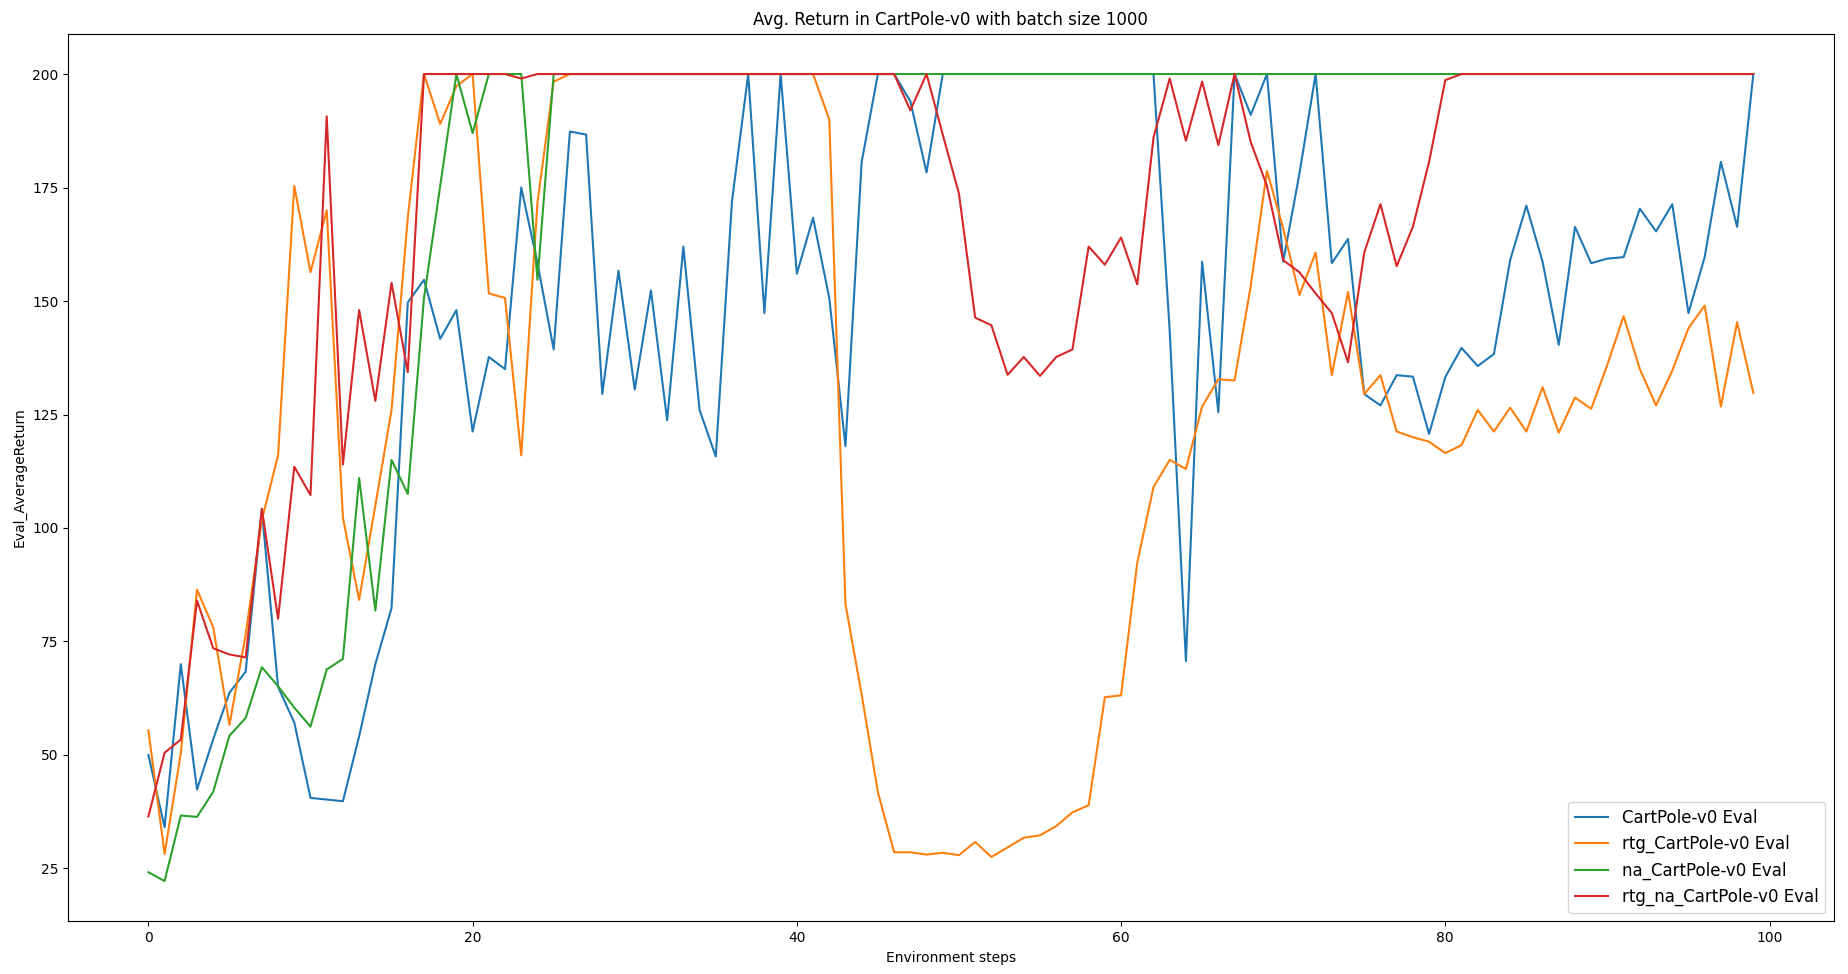
\includegraphics[width=0.9\linewidth]{hw2_pg_small_batch.png} 
		\caption{1000 batch size}
		\label{fig:1}
	\end{subfigure}
	\begin{subfigure}{0.48\textwidth}
		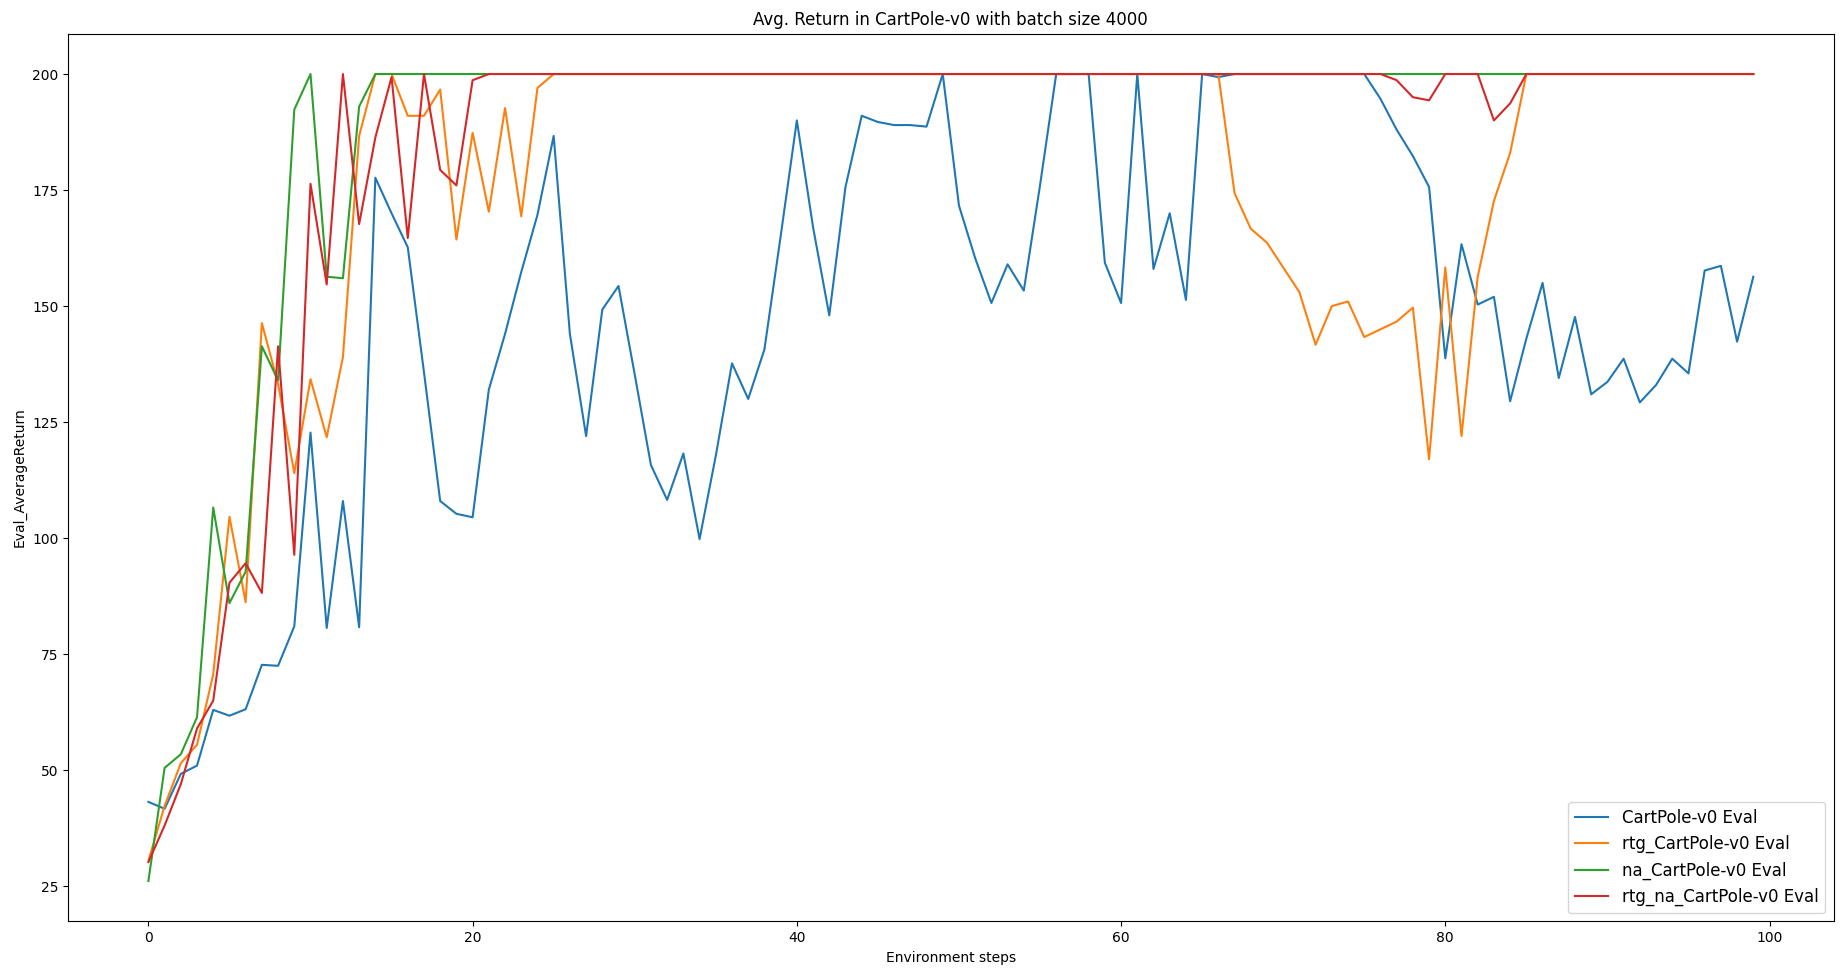
\includegraphics[width=0.9\linewidth]{hw2_pg_large_batch.png}
		\caption{4000 batch size}
		\label{fig:2}
	\end{subfigure}
\end{figure}


\item Answer the following questions briefly: 
    \begin{itemize}
    \item \textbf{Q1.} Which value estimator has better performance without advantage normalization: the trajectory-centric one, or the one using reward-to-go? \\
    \textbf{A1.} In small batch size, it is hard to tell the reward-to-go(\textcolor{yellow}{Yellow}) is definitely better than the trajectory-centric one(\textcolor{blue}{Blue}). However, in large batch size, the reward-to-go shows better performance.
    \item \textbf{Q2.} Did advantage normalization help? \\
    \textbf{A2.} Yes. Overall, the advantage normalization helps to stabilize the learning process.
    \item \textbf{Q3.} Did the batch size make an impact? \\
    \textbf{A3.} Yes. In large batch size, the learning process is more stable and the performance is better.
    \end{itemize}
\end{itemize}
\textbf{NOTE.} The exact command line configurations for each experiment are provided in \href{https://github.com/ChanJoon/CS285_hw_fall2023/tree/main/hw2/README.md}{README.md.}

\newpage\section{Neural Network Baseline}
\begin{itemize}
    \item Plot a learning curve for the baseline loss.
    \begin{figure}[H]
        \centering
        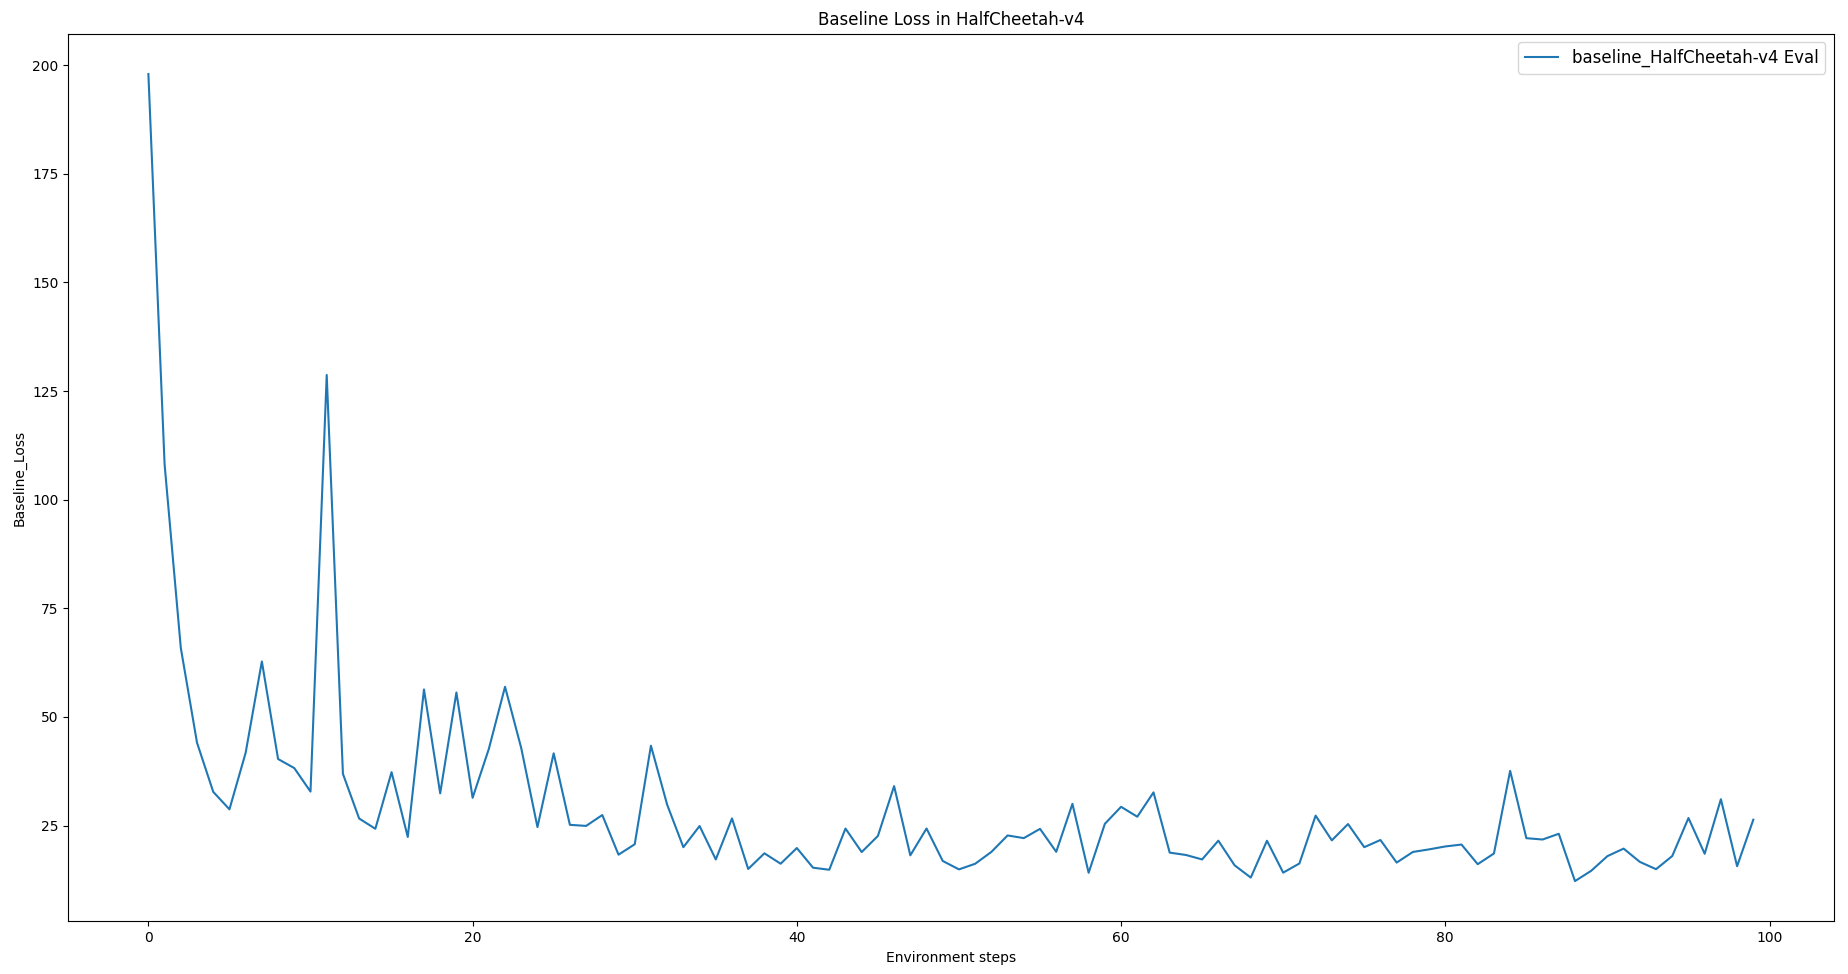
\includegraphics[width=0.6\textwidth]{hw2_baseline_loss.png}
    \end{figure}
    \item Plot a learning curve for the eval return. You should expect to achieve an average return over 300 for the baselined version.
    \begin{figure}[H]
        \centering
        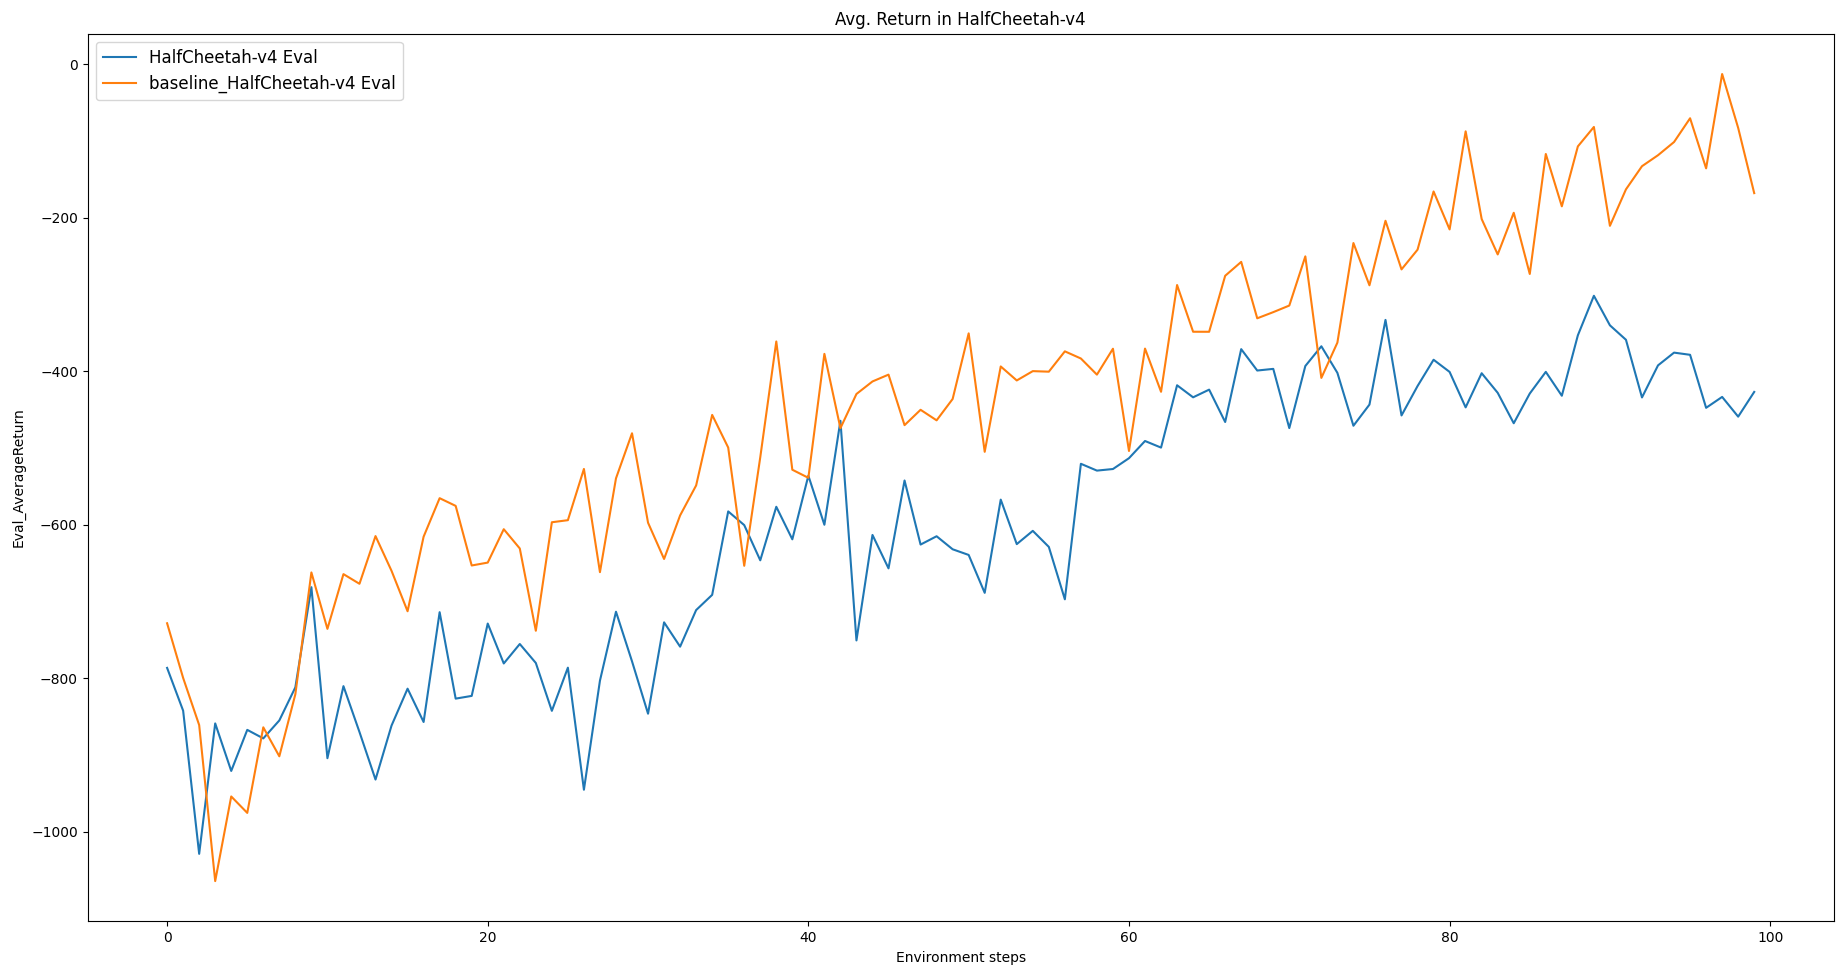
\includegraphics[width=0.6\textwidth]{hw2_baseline_return.png}
    \end{figure}
    With the given command-line arguments, it failed to achieve the average return over 300. 
    \begin{figure}[H]
        \centering
        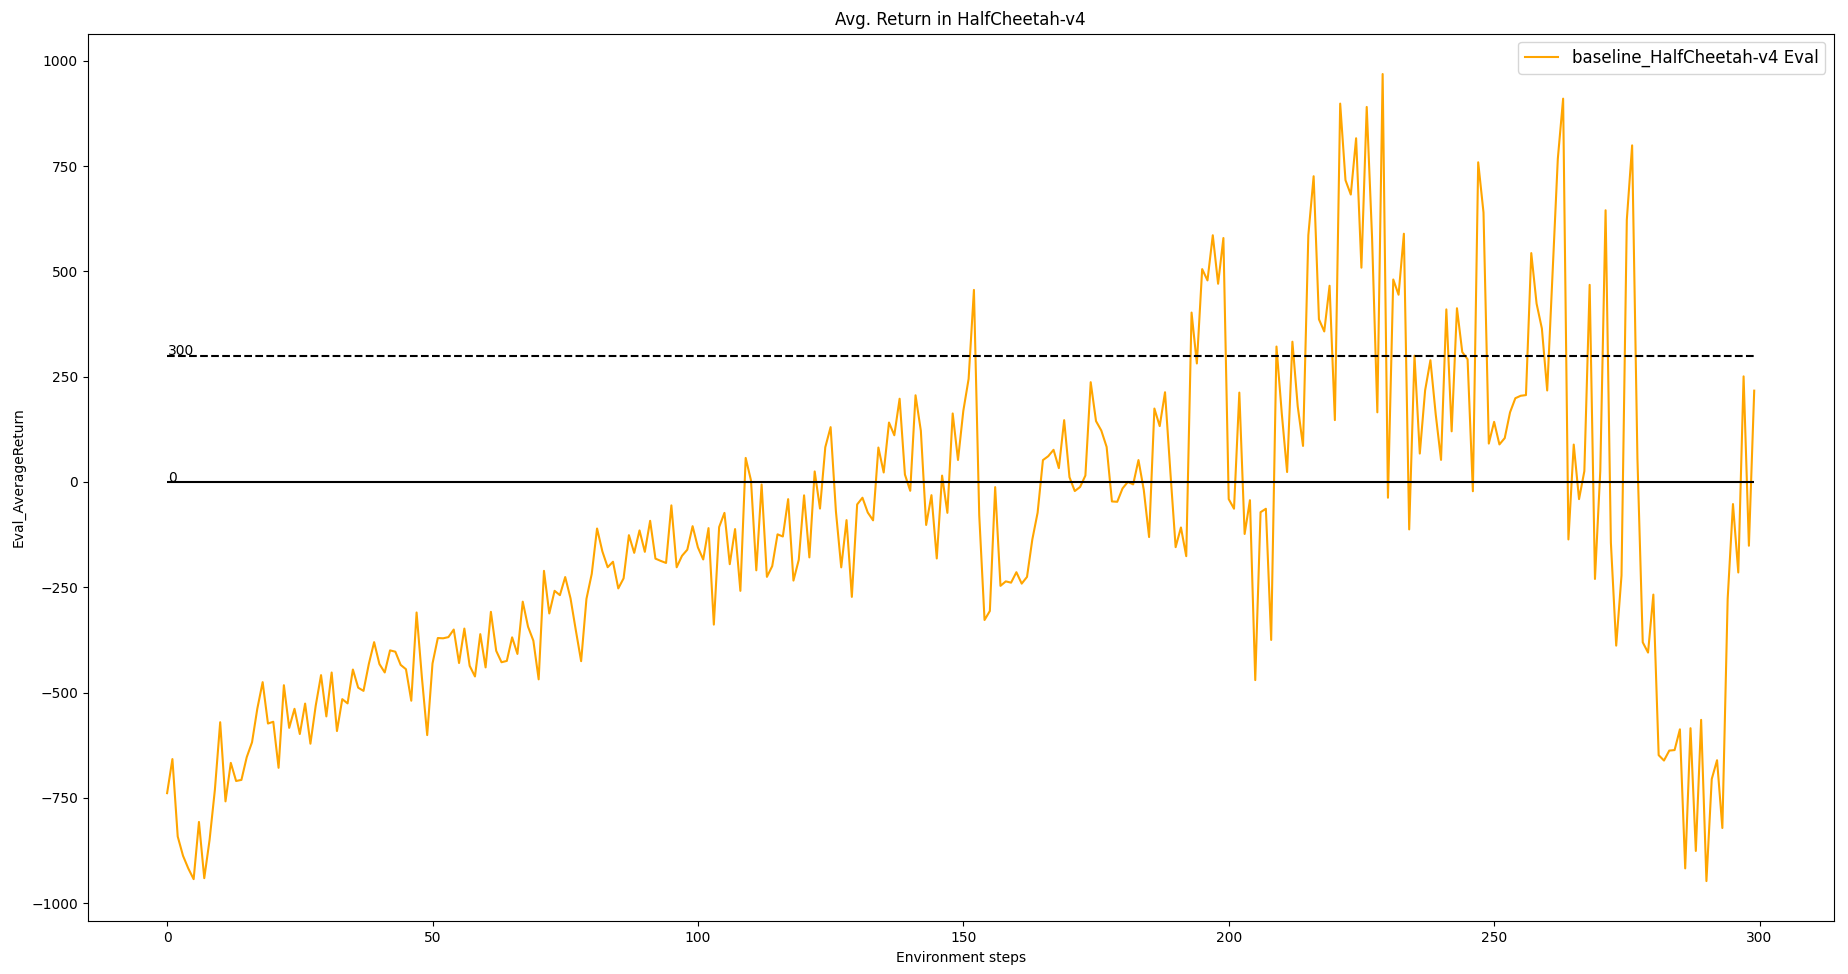
\includegraphics[width=0.6\textwidth]{hw2_baseline_loss_300.png}
    \end{figure}
    But as we can see, with 300 steps, it achieved the average return almost 300.
    \item Run another experiment with a decreased number of baseline gradient steps (\verb|-bgs|) and/or baseline learning rate (\verb|-blr|). How does this affect (a) the baseline learning curve and (b) the performance of the policy?
    \begin{figure}[H]
        \centering
        \begin{subfigure}{0.48\textwidth}
            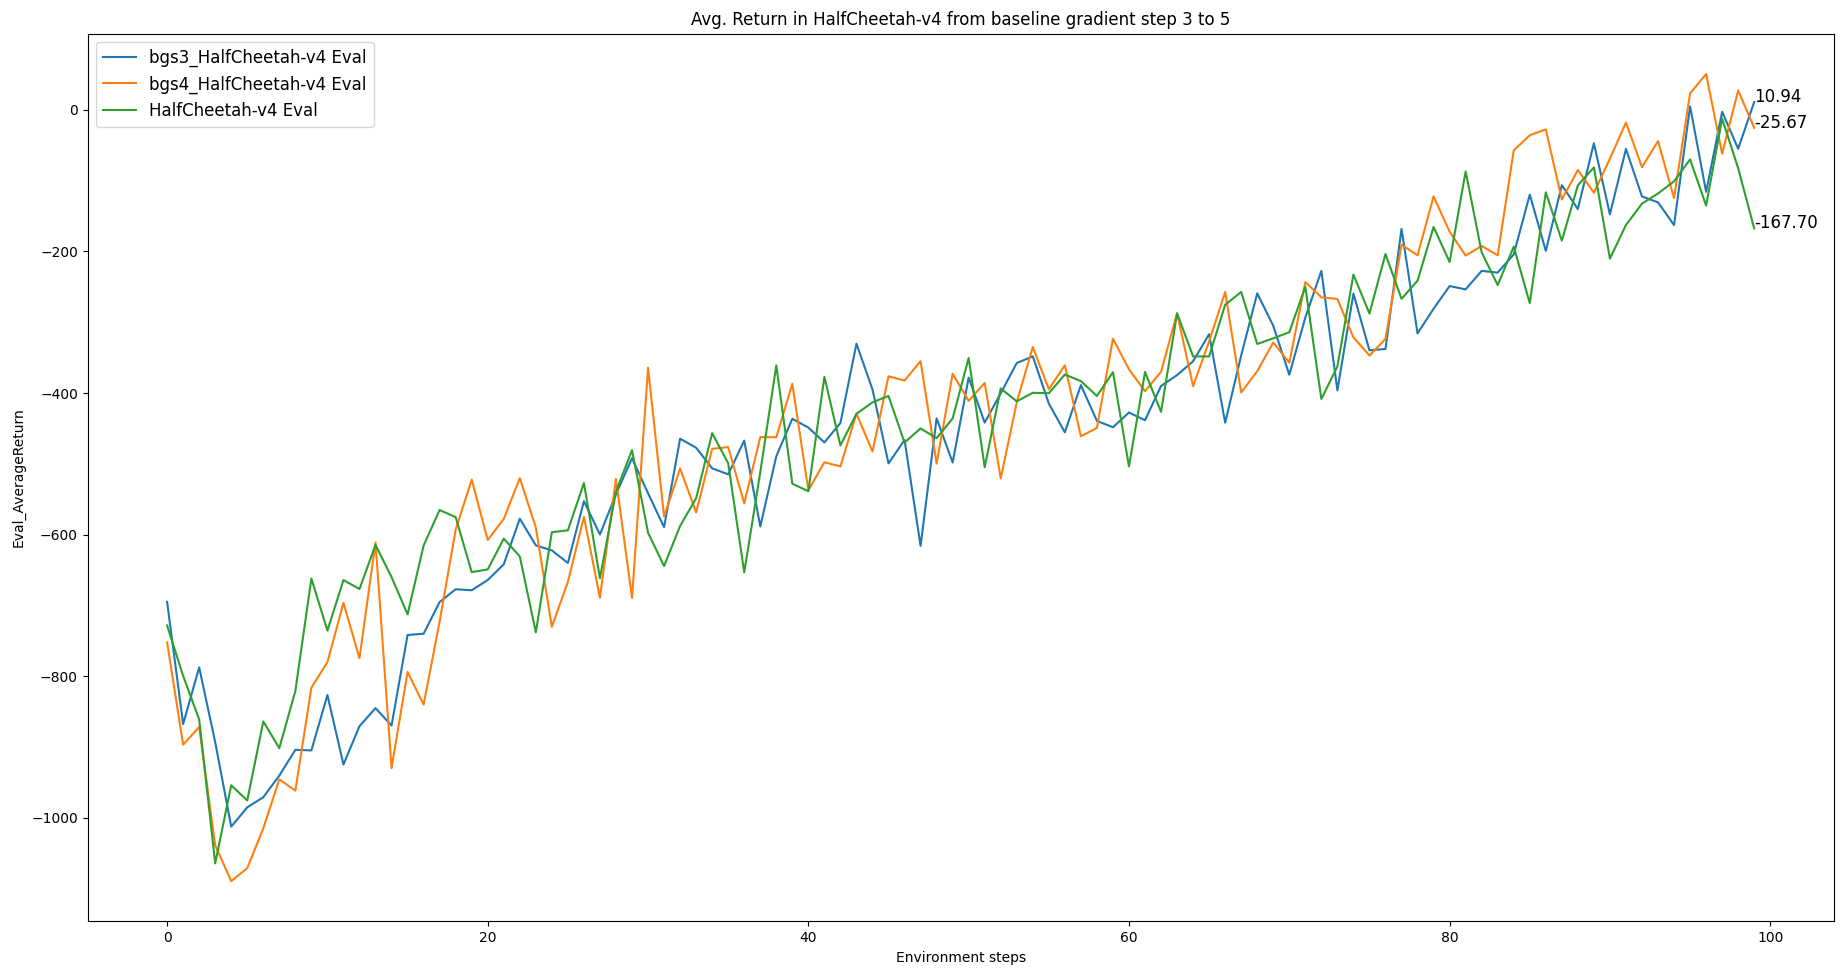
\includegraphics[width=0.9\linewidth]{hw2_baseline_bgs.png} 
            \caption{Baseline gradient step}
            \label{fig:3}
        \end{subfigure}
        \begin{subfigure}{0.48\textwidth}
            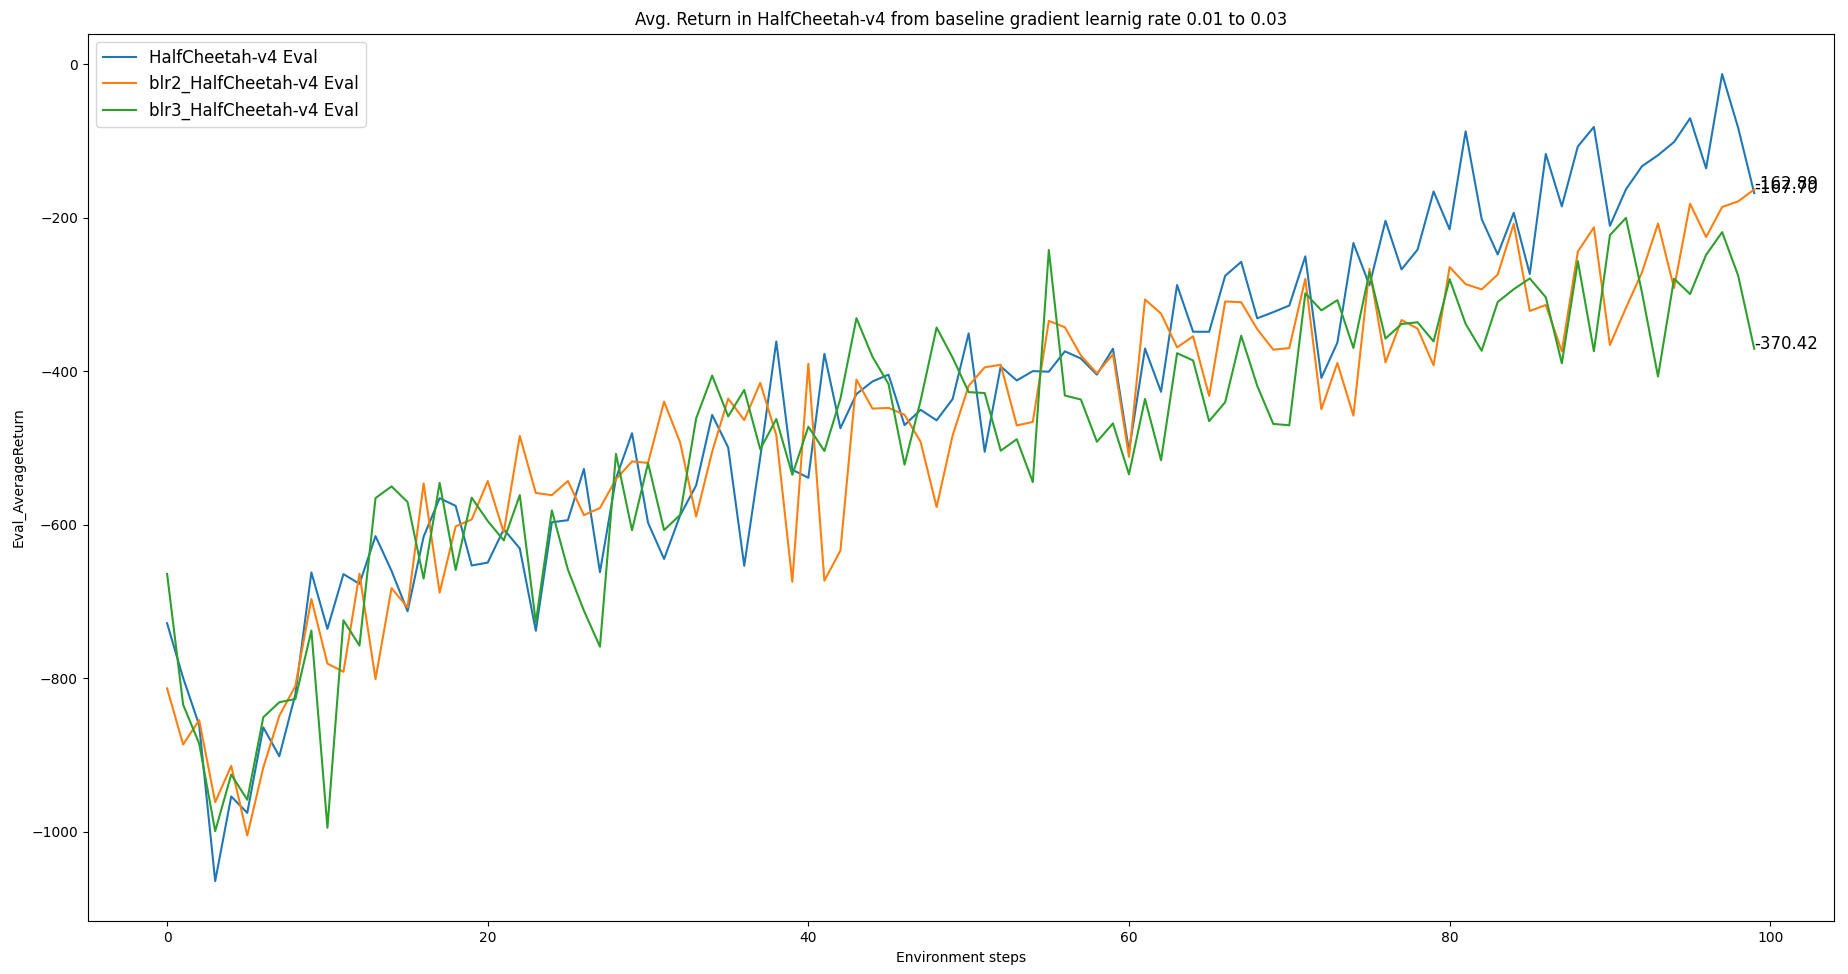
\includegraphics[width=0.9\linewidth]{hw2_baseline_blr.png}
            \caption{Baseline learning rate}
            \label{fig:4}
        \end{subfigure}
    \end{figure}
    Interestingly, the smaller baseline gradient step shows better performance than the larger one. And as we know, the smaller baseline learning rate shows better performance than the larger one.

    But this is just 3 experiments, so it is hard to tell the exact relationship between the baseline gradient step and the baseline learning rate.
    \item \textbf{Optional:} Add \verb|-na| back to see how much it improves things. Also, set \verb|video_log_freq 10|, then open TensorBoard and go to the ``Images'' tab to see some videos of your HalfCheetah walking along!
    
    Attached video files are in \href{https://github.com/ChanJoon/CS285_hw_fall2023/tree/main/hw2/README.md}{README.md.} But as you can see, it is not walking expectedly.
\end{itemize}

\newpage\section{Generalized Advantage Estimation}
\begin{itemize}
    \item Provide a single plot with the learning curves for the \verb|LunarLander-v2| experiments that you tried. Describe in words how $\lambda$ affected task performance. The run with the best performance should achieve an average score close to 200 (180+).
    \item Consider the parameter $\lambda$. What does $\lambda = 0$ correspond to? What about $\lambda = 1$? Relate this to the task performance in \verb|LunarLander-v2| in one or two sentences.
    \begin{figure}[H]
        \centering
        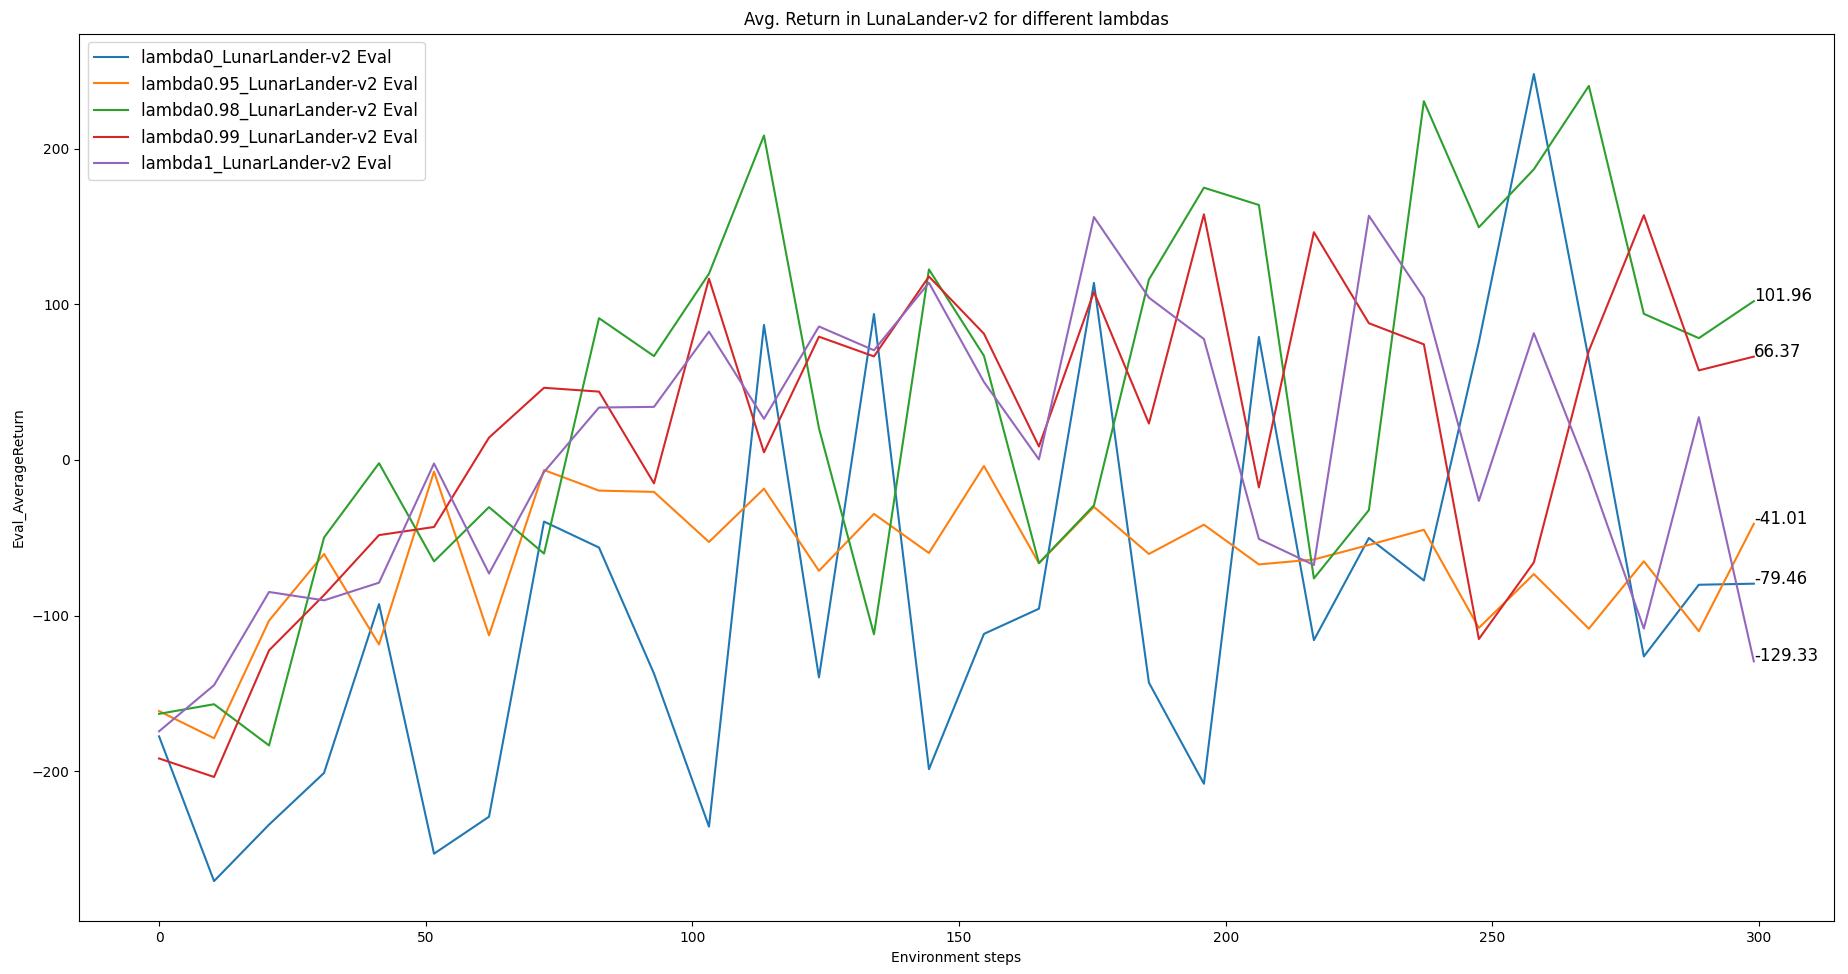
\includegraphics[width=0.9\textwidth]{hw2_lambda.png}
    \end{figure}
    Please note that this plot is smoothed with interpolation due to the large variance of the return. As we can see, the $\lambda = 0.98$ and $0.99$ shows the best performance. The $\lambda = 0$ corresponds to the one-step TD error for estimating the advantage function, and the $\lambda = 1$ corresponds to the Monte Carlo estimate.
\end{itemize}

\newpage\section{Hyperparameter Tuning}
\begin{enumerate}
    \item Provide a set of hyperparameters that achieve high return on \verb|InvertedPendulum-v4| in as few environment steps as possible.
    \item Show learning curves for the average returns with your hyperparameters and with the default settings, with environment steps on the $x$-axis. Returns should be averaged over 5 seeds.
\end{enumerate}
\begin{figure}[H]
    \centering
    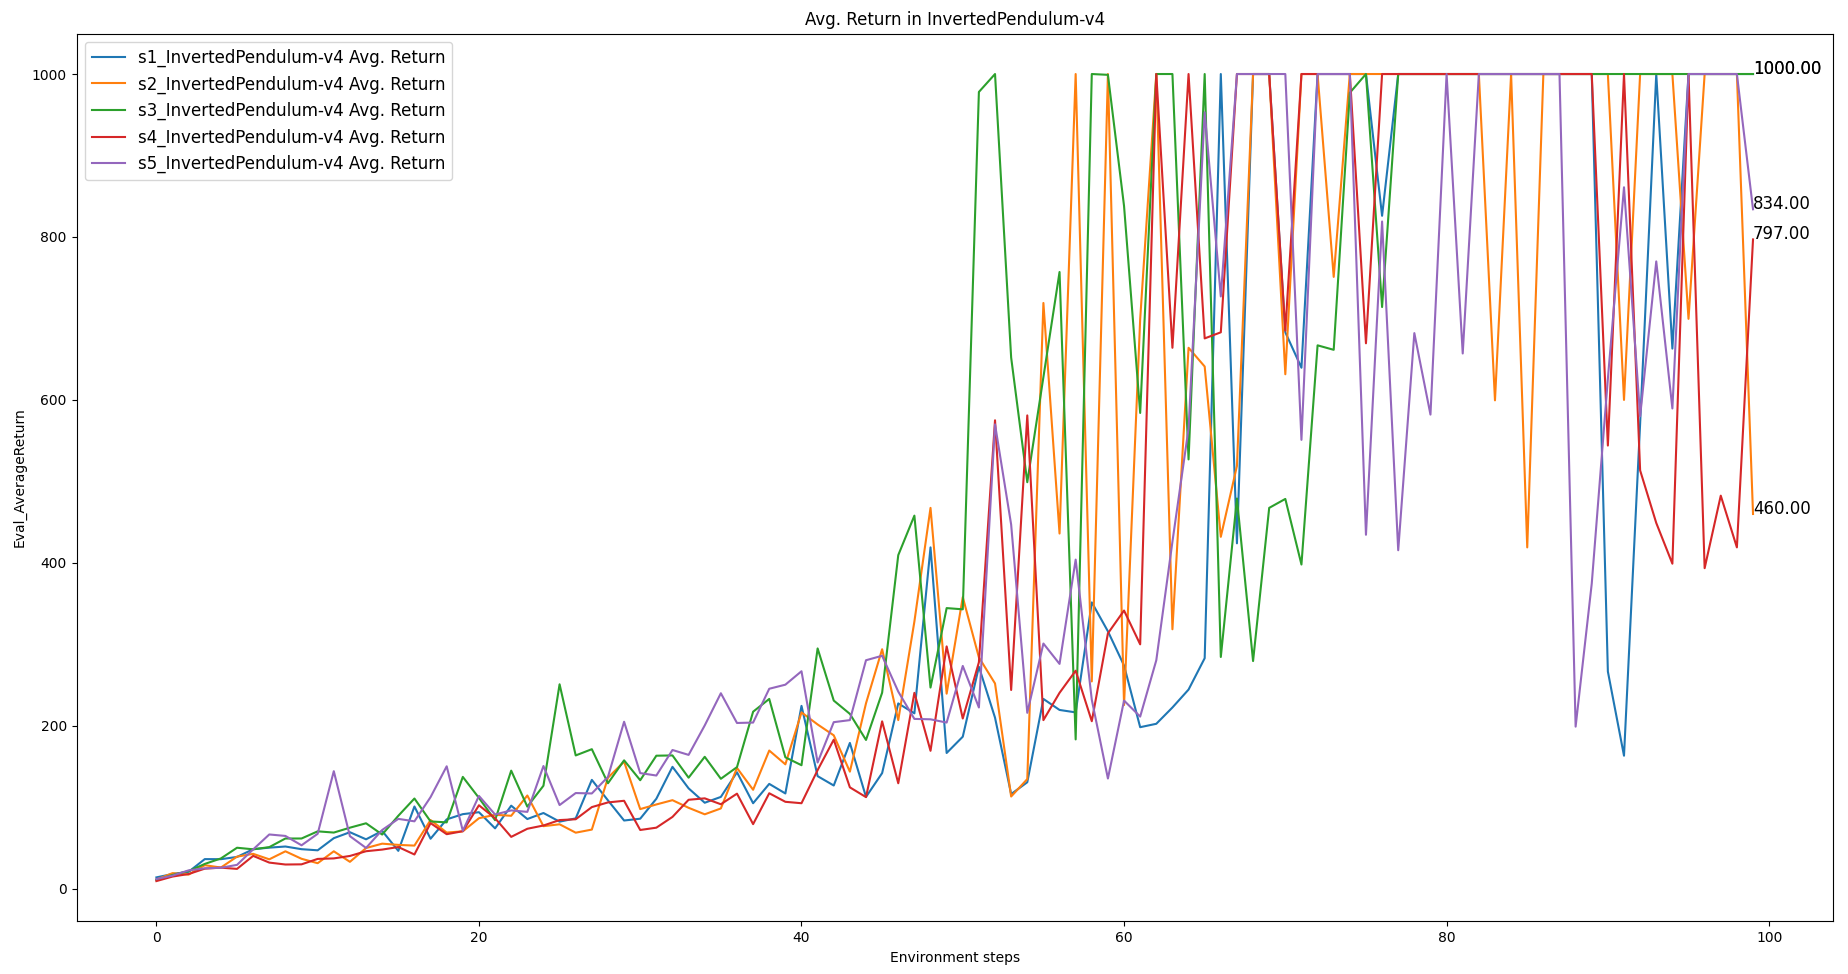
\includegraphics[width=0.9\textwidth]{hw2_hyperparameter.png}
\end{figure}

\newpage\section{(Extra Credit) Humanoid}
\begin{enumerate}
    \item Plot a learning curve for the Humanoid-v4 environment. You should expect to achieve an average return of at least 600 by the end of training. Discuss what changes, if any, you made to complete this problem (for example: optimizations to the original code, hyperparameter changes, algorithmic changes).
\end{enumerate}

\newpage\section{Analysis}
\label{sec:analysis}
Consider the following infinite-horizon MDP:
% https://q.uiver.app/#q=WzAsMixbMCwwLCJzIl0sWzAsMSwic19GIl0sWzAsMSwiYV8yIl1d
\[\begin{tikzcd}
	s_1 & {s_F}
	\arrow["{a_2}", from=1-1, to=1-2]
    \arrow["{a_1}", loop left, from=1-1, to=1-1]
\end{tikzcd}\]
\newcommand{\Rmax}[0]{R_{\textrm{max}}}
\newcommand{\E}[0]{\mathbb{E}}
\newcommand{\var}[0]{\textrm{Var}}
\crefname{question}{part}{parts}
\Crefname{question}{Part}{Parts}
\newcommand\question[1][]{\item\refstepcounter{subsection}\label[question]{#1}}

At each step, the agent stays in state $s_1$ and receives reward 1 if it takes action $a_1$, and receives reward 0 and terminates the episode otherwise.
Parametrize the policy as stationary (not dependent on time) with a single parameter:
\[\pi_\theta(a_1|s_1) = \theta, \pi_\theta(a_2|s_1) = 1-\theta\]

\begin{enumerate}
\question[sec:analysis1] Applying policy gradients
\begin{enumerate}
    \item Use policy gradients to compute the gradient of the expected return $R(\tau)$ with respect to the parameter $\theta$. \textbf{Do not use discounting.}

    \textbf{Hint}: to compute $\sum_{k=1}^\infty k\alpha^{k-1}$, you can write:
    \[\sum_{k=1}^\infty k\alpha^{k-1} = \sum_{k=1}^\infty \frac{d}{d\alpha}\alpha^k = \frac{d}{d\alpha}\sum_{k=1}^\infty\alpha^k\]

\textbf{Solution:} The policy gradient $\nabla_\theta J(\theta)$ is given by $\nabla_\theta \E_{\tau\sim\pi_\theta} R(\tau) = \E_{\tau\sim\pi_\theta} \nabla_\theta \log \pi_\theta(\tau) R(\tau)$. In our case, $\nabla_\theta \log \pi_\theta(a_1|s_1) = \nabla_\theta \log \theta = \frac{1}{\theta}$.

the expecte return $R(\tau)$ is given by $\sum_{k=1}^\infty k\theta^{k-1}(1-\theta)$ for $\tau=s_1,a_1,\ldots,s_1,a_2$ at step $k$. With the Hint provided, \[\sum_{k=1}^\infty k\theta^{k-1} = \frac{d}{d\theta}\sum_{k=1}^\infty \theta^k = \frac{d}{d\theta}\frac{\theta}{1-\theta} = \frac{1}{{(1-\theta)}^2}\] and \[R(\tau) = \sum_{k=1}^\infty k\theta^{k-1}(1-\theta) = \frac{1}{1-\theta}\]

Now we can say the gradient of the expected return is given by \[\nabla_\theta J(\theta) = \frac{1}{\theta(1-\theta)}\]

    \item \label{exact_gradient} Compute the expected return of the policy $\E_{\tau \sim \pi_\theta} R(\tau)$ directly. Compute the gradient of this expression with respect to $\theta$ and verify that this matches the policy gradient.

\textbf{Solution:} For $\tau = s_1, a_1, \ldots, s_1, a_2$ at step $k$, the expected return of the policy $J(\theta)$ is given by \[J(\theta) = \E_{\tau\sim \pi_\theta} R(\tau) = \frac{1}{1-\theta}\] The gradient of this expression with respect to $\theta$ is given by \[\nabla_\theta J(\theta) = \frac{1}{{(1-\theta)}^2}\], which does not match the policy gradient computed in part 1 (a).

\end{enumerate}
\newpage
\question[sec:analysis2] Compute the variance of the policy gradient in closed form and describe the properties of the variance with respect to $\theta$. For what value(s) of $\theta$ is variance minimal? Maximal? (Once you have an exact expression for the variance you can eyeball the min/max).

\textbf{Hint:}  Once you have it expressed as a sum of terms $P(\theta)/Q(\theta)$ where $P$ and $Q$ are polynomials, you can use a symbolic computing program (Mathematica, SymPy, etc) to simplify to a single rational expression.

\textbf{Solution:}

\newpage
\question[sec:analysis3] Apply return-to-go as an advantage estimator.
\begin{enumerate}
    \item Write the modified policy gradient and confirm that it is unbiased.

\textbf{Solution:}

    \item Compute the variance of the return-to-go policy gradient and plot it on $[0, 1]$ alongside the variance of the original estimator.

\textbf{Solution:}

\end{enumerate}
\newpage
\question[sec:analysis4] Consider a finite-horizon $H$-step MDP with sparse reward:
% https://q.uiver.app/#q=WzAsNixbMCwwLCJzXzEiXSxbMSwwLCJzXzIiXSxbMiwwLCJzXzMiXSxbMiwxLCJzX0YiXSxbMywwLCJcXGRvdHMiXSxbNCwwLCJzX0giXSxbMCwxLCJhXzEiXSxbMSwyLCJhXzEiXSxbMCwzLCJhXzIiLDJdLFsyLDQsImFfMSJdLFs0LDVdLFsxLDMsImFfMiJdLFsyLDMsImFfMiIsMV0sWzQsMywiYV8yIiwxXV0=
\[\begin{tikzcd}
	{s_1} & {s_2} & {s_3} & \dots & {s_H} \\
	&& {s_F}
	\arrow["{a_1}", from=1-1, to=1-2]
	\arrow["{a_1}", from=1-2, to=1-3]
	\arrow["{a_2}"', from=1-1, to=2-3]
	\arrow["{a_1}", from=1-3, to=1-4]
	\arrow[from=1-4, to=1-5]
	\arrow["{a_2}", from=1-2, to=2-3]
	\arrow["{a_2}"{description}, from=1-3, to=2-3]
	\arrow["{a_2}"{description}, from=1-4, to=2-3]
\end{tikzcd}\]

The agent receives reward $\Rmax$ if it arrives at $s_H$ and reward $0$ if it arrives at $s_F$ (a terminal state). In other words, the return for a trajectory $\tau$ is given by:
\[R(\tau) = \begin{cases}1 & \tau \textrm{ ends at } s_H \\ 0 & \tau \textrm{ ends at } s_F \end{cases}\]
Using the same policy parametrization as above, consider off-policy policy gradients via importance sampling. Assume we want to compute policy gradients for a policy $\pi_\theta$ with samples drawn from $\pi_{\theta'}$.
\begin{enumerate}
    \item Write the policy gradient with importance sampling.

    \item Compute its variance.

\end{enumerate}

\end{enumerate}

\newpage\section{Survey}
\label{sec:survey}
Please estimate, in minutes, for each problem, how much time you spent (a) writing code and (b) waiting for the results. This will help us calibrate the difficulty for future homeworks. 
\begin{itemize}
    \item \textbf{Policy Gradients:}
    \item \textbf{Neural Network Baseline:}
    \item \textbf{Generalized Advantage Estimation:}
    \item \textbf{Hyperparameters and Sample Efficiency:}
    \item \textbf{Humanoid:}
    \item \textbf{Humanoid:}
    \item \textbf{Analysis -- applying policy gradients:}
    \item \textbf{Analysis -- PG variance:}
    \item \textbf{Analysis -- return-to-go:}
    \item \textbf{Analysis -- importance sampling:}
\end{itemize}

\end{document}
